%%%%%%%%%%%%%%%%%%%%%%%%%%%%%%%%%%%
%This is the LaTeX ARTICLE template for RSC journals
%Copyright The Royal Society of Chemistry 2016
%%%%%%%%%%%%%%%%%%%%%%%%%%%%%%%%%%%

\documentclass[twoside,twocolumn,9pt]{article}
\usepackage{extsizes}
\usepackage[super,sort&compress,comma]{natbib} 
\usepackage[version=3]{mhchem}
\usepackage[left=1.5cm, right=1.5cm, top=1.785cm, bottom=2.0cm]{geometry}
\usepackage{balance}
\usepackage{times,mathptmx}
\usepackage{sectsty}
\usepackage{graphicx} 
\usepackage{lastpage}
\usepackage[format=plain,justification=justified,singlelinecheck=false,font={stretch=1.125,small,sf},labelfont=bf,labelsep=space]{caption}
\usepackage{float}
\usepackage{fancyhdr}
\usepackage{fnpos}
\usepackage[english]{babel}
\usepackage{array}
\usepackage{droidsans}
\usepackage{charter}
\usepackage[T1]{fontenc}
\usepackage[usenames,dvipsnames]{xcolor}
\usepackage{setspace}
\usepackage[compact]{titlesec}
%%%Please don't disable any packages in the preamble, as this may cause the template to display incorrectly.%%%
\usepackage[obeyFinal]{easy-todo}
\usepackage{url}
\usepackage{rotating}


\usepackage{epstopdf}%This line makes .eps figures into .pdf - please comment out if not required.

\definecolor{cream}{RGB}{222,217,201}

\begin{document}

\renewcommand{\thefigure}{S\arabic{figure}}
\pagestyle{fancy}
\thispagestyle{plain}
%\fancypagestyle{plain}{

%%%HEADER%%%
%\fancyhead[C]{\includegraphics[width=18.5cm]{head_foot/header_bar}}
%\fancyhead[L]{\hspace{0cm}\vspace{1.5cm}\includegraphics[height=30pt]{head_foot/journal_name}}
%\fancyhead[R]{\hspace{0cm}\vspace{1.7cm}\includegraphics[height=55pt]{head_foot/RSC_LOGO_CMYK}}
%\renewcommand{\headrulewidth}{0pt}
%}
%%%END OF HEADER%%%

%%%PAGE SETUP - Please do not change any commands within this section%%%
\makeFNbottom
\makeatletter
\renewcommand\LARGE{\@setfontsize\LARGE{15pt}{17}}
\renewcommand\Large{\@setfontsize\Large{12pt}{14}}
\renewcommand\large{\@setfontsize\large{10pt}{12}}
\renewcommand\footnotesize{\@setfontsize\footnotesize{7pt}{10}}
\makeatother

\renewcommand{\thefootnote}{\fnsymbol{footnote}}
\renewcommand\footnoterule{\vspace*{1pt}% 
\color{cream}\hrule width 3.5in height 0.4pt \color{black}\vspace*{5pt}} 
\setcounter{secnumdepth}{5}

\makeatletter 
\renewcommand\@biblabel[1]{#1}            
\renewcommand\@makefntext[1]% 
{\noindent\makebox[0pt][r]{\@thefnmark\,}#1}
\makeatother 
\renewcommand{\figurename}{\small{Fig.}~}
\sectionfont{\sffamily\Large}
\subsectionfont{\normalsize}
\subsubsectionfont{\bf}
\setstretch{1.125} %In particular, please do not alter this line.
\setlength{\skip\footins}{0.8cm}
\setlength{\footnotesep}{0.25cm}
\setlength{\jot}{10pt}
\titlespacing*{\section}{0pt}{4pt}{4pt}
\titlespacing*{\subsection}{0pt}{15pt}{1pt}
%%%END OF PAGE SETUP%%%

%%%FOOTER%%%
%\fancyfoot{}
%\fancyfoot[LO,RE]{\vspace{-7.1pt}\includegraphics[height=9pt]{head_foot/LF}}
%\fancyfoot[CO]{\vspace{-7.1pt}\hspace{13.2cm}\includegraphics{head_foot/RF}}
%\fancyfoot[CE]{\vspace{-7.2pt}\hspace{-14.2cm}\includegraphics{head_foot/RF}}
%\fancyfoot[RO]{\footnotesize{\sffamily{1--\pageref{LastPage} ~\textbar  \hspace{2pt}\thepage}}}
%\fancyfoot[LE]{\footnotesize{\sffamily{\thepage~\textbar\hspace{3.45cm} 1--\pageref{LastPage}}}}
%\fancyhead{}
\renewcommand{\headrulewidth}{0pt} 
\renewcommand{\footrulewidth}{0pt}
\setlength{\arrayrulewidth}{1pt}
\setlength{\columnsep}{6.5mm}
\setlength\bibsep{1pt}
%%%END OF FOOTER%%%

%%%FIGURE SETUP - please do not change any commands within this section%%%
\makeatletter 
\newlength{\figrulesep} 
\setlength{\figrulesep}{0.5\textfloatsep} 

\newcommand{\topfigrule}{\vspace*{-1pt}% 
\noindent{\color{cream}\rule[-\figrulesep]{\columnwidth}{1.5pt}} }

\newcommand{\botfigrule}{\vspace*{-2pt}% 
\noindent{\color{cream}\rule[\figrulesep]{\columnwidth}{1.5pt}} }

\newcommand{\dblfigrule}{\vspace*{-1pt}% 
\noindent{\color{cream}\rule[-\figrulesep]{\textwidth}{1.5pt}} }

\makeatother
%%%END OF FIGURE SETUP%%%

%%%TITLE, AUTHORS AND ABSTRACT%%%
\twocolumn[
  \begin{@twocolumnfalse}
\vspace{3cm}
\sffamily
\begin{tabular}{m{4.5cm} p{13.5cm} }

 & \noindent\LARGE{\textbf{Supplementary Information: Molecular electrometer and binding of cations to phospholipid bilayers$^\dag$}} \\%Article title goes here instead of the text "This is the title"
\vspace{0.3cm} & \vspace{0.3cm} \\

 & \noindent\large{Andrea Catte,\textit{$^{a\ddag}$} Mykhailo Girych,\textit{$^{b}$} Matti Javanainen,\textit{$^{cd}$} Claire Loison,\textit{$^{e}$} Josef Melcr,\textit{$^{fg}$} Markus S. Miettinen,\textit{$^{hi}$} Luca Monticelli,\textit{$^{j}$} Jukka M{\"a}{\"a}tt{\"a},\textit{$^{k}$} Vasily S. Oganesyan,\textit{$^{a}$} O. H. Samuli Ollila,\textit{$^{\ast b}$} Joona Tynkkynen\textit{$^{c}$} and Sergey Vilov\textit{$^{e}$}
} \\%Author names go here instead of "Full name", etc.


\end{tabular}

 \end{@twocolumnfalse} \vspace{0.6cm}

  ]
%%%END OF TITLE, AUTHORS AND ABSTRACT%%%

%%%FONT SETUP - please do not change any commands within this section
\renewcommand*\rmdefault{bch}\normalfont\upshape
\rmfamily
\section*{}
\vspace{-1cm}


%%%FOOTNOTES%%%

\footnotetext{\textit{$^{a}$~School of Chemistry, University of East Anglia, Norwich, NR4 7TJ, United Kingdom}}
\footnotetext{\textit{$^{b}$~Department of Neuroscience and Biomedical Engineering, Aalto University, Espoo, Finland}}
\footnotetext{\textit{$^{c}$~Department of Physics, Tampere University of Technology, Tampere, Finland}}
\footnotetext{\textit{$^{d}$~Department of Physics, University of Helsinki, Helsinki, Finland}}
\footnotetext{\textit{$^{e}$~Univ Lyon, Universit{\'e} Claude Bernard Lyon 1, CNRS, Institut Lumi{\'e}re Mati{\'e}re, F-69622, LYON, France}}
\footnotetext{\textit{$^{f}$~Institute of Organic Chemistry and Biochemistry, Czech Academy of Sciences, Flemingovo n{\'a}m. 2, 16610 Prague 6, Czech Republic}}
\footnotetext{\textit{$^{g}$~Charles University in Prague, Faculty of Mathematics and Physics, Ke Karlovu 3, 121 16 Prague 2, Czech Republic}}
\footnotetext{\textit{$^{h}$~Fachbereich Physik, Freie Universit\"at Berlin, Berlin, Germany}}
\footnotetext{\textit{$^{i}$~Max Planck Institute of Colloids and Interfaces, Department of Theory and Bio-Systems, Potsdam, Germany}}
\footnotetext{\textit{$^{j}$~Institut de Biologie et Chimie des Prot{\'e}ines (IBCP), CNRS UMR 5086, Lyon, France}}
\footnotetext{\textit{$^{k}$~Department of Chemistry, Aalto University, Espoo, Finland}}
\footnotetext{\textit{$^{\ast}${\bf Author to whom correspondence may be addressed. E-mail: samuli.ollila@aalto.fi.}}}


%\footnotetext{\textit{$^{b}$~Address, Address, Town, Country. Fax: XX XXXX XXXX; Tel: XX XXXX XXXX; E-mail: xxxx@aaa.bbb.ccc}} }}



%Please use \dag to cite the ESI in the main text of the article.
%If you article does not have ESI please remove the the \dag symbol from the title and the footnotetext below.
%\footnotetext{\dag~Electronic Supplementary Information (ESI) available: %[details of any supplementary information available should be included here]. 
%8 figures, detailed technical discussion and simulation details.
%See DOI: 10.1039/b000000x/}
%additional addresses can be cited as above using the lower-case letters, c, d, e... If all authors are from the same address, no letter is required

\footnotetext{\ddag~The authors are listed in alphabetical order. 
%Additional footnotes to the title and authors can be included \textit{e.g.}\ `Present address:' 
%or `These authors contributed equally to this work' as above using the symbols: \ddag, \textsection, 
%and \P. Please place the appropriate symbol next to the author's name and include a \texttt{\textbackslash footnotetext} 
%entry in the the correct place in the list.
}


%%%END OF FOOTNOTES%%%

%%%MAIN TEXT%%%%


%\begin{center}
%\part*{SUPPLEMENTARY INFORMATION}
%\end{center}
\section{Ca$^{2+}$ binding equilibration times}
To estimate the times required to equilibrate the amount of bound Ca$^{2+}$ in lipid bilayer,
simulations containing 450~mM CaCl$_2$ were ran with CHARMM36 and Slipids  for 2~$\mu$s (Fig.~\ref{longruns}).
\begin{figure}[h]
  \centering
  \includegraphics[width=8cm]{../Fig/bindingINlongRUNS.eps} 
  \caption{\label{longruns}
    Number of bound Ca$^{2+}$ during 2~$\mu$s simulations with CHARMM36 and Slipids.
}
\end{figure}
There was a clear increase in ion binding up to 1000~ns in CHARMM36 and 700~ns in Slipids,
and a moderate increase even after this. This was also reflected in the CHARMM36 results of Fig.~2 in the main text, where
the long CHARMM36 simulation with $[$CaCl$_2]=450$~mM showed lower order parameters than shorter simulations
with  $[$CaCl$_2]>450$~mM, in line
with the higher (see Fig.~\ref{CAdensities})  ion binding in the (more equilibrated) long simulation. 

These results suggest that in the other simulations the Ca$^{2+}$ binding affinities 
may also be underestimated due to insufficient equilibration times. While this should be taken into account in more careful studies,
it does not interfere with our key conclusion that Ca$^{2+}$ binding is most likely overestimated in all the
models --- except in CHARMM36 with the heptahydrated Ca$^{2+}$ by Yoo et al. \cite{yoo16},
for which the number of Ca$^{2+}$ ions on the coordination shell of lipid oxygens (the measurable shown in Fig.~\ref{longruns})
would remain strictly at zero at all times, as each calcium is explicitly bound to a set of seven water molecules.


\section{Change of choline order parameters as a function of bound cation charge}


To demonstrate that also in current MD simulations the molecular electrometer works as Seelig and coworkers proposed in the 1980's (that is, there is a direct relationship between the changes in the choline $\beta$ and $\alpha$ segment order parameters and the amount of penetrated charge), we calculated the bound cation charge and the corresponding order parameter change separately for each leaflet in several MD simulation systems.

As in reality ions have continuum density distributions, any division to bound and non-bound ions is somewhat artificial,
and thus the choice of parameters describing ion partitioning is more or less ambiguous.
We chose to integrate the cation charge distribution from the centre of the membrane until a certain predefined limit. Three limits were tested:
until the g$_3$-carbon (Fig.~\ref{electrometer_g3}), until the phosphorus (Fig.~3 in the main text), and until the $\alpha$-carbon (Fig.~\ref{electrometer_ca}) density maximum. Although phosphorus seems to be the most intuitive choice, comparison of these three plots shows that the conclusions we drew here did not depend on the chosen limit.
That said, we must stress that the slopes of the curves depend {\bf strongly} on the chosen limit; therefore, one should be very careful when comparing them to one another or to experimental data --- a given limit might or might not match with what is considered 'bound' in an experiment.
%To put it in other words, we can affect the slopes of the simulation curves by our choice of the integration limit, whereas the experimental slope will not be affected. This has a potential of us introducing an unconscious bias on the one hand, and on the other hand people looking at the plot might conclude one FF to be better matching the experiments than some other, although this might not be the case (both because the OPs at zero bound charge in the simulations are not correct and because of this additional effect on the slope coming from the choice of the integration limit.)

\begin{figure}[t]
  \centering
  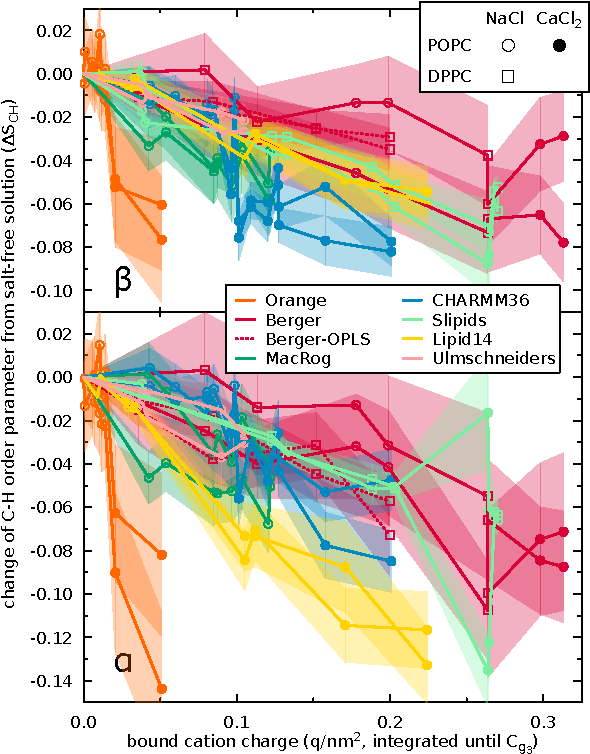
\includegraphics[width=8.6cm]{../Fig/dOP_vs_boundCationCharge_Cg3.pdf}
  \caption{\label{electrometer_g3}
    Change of order parameters (from salt-free solution) of the $\beta$ and $\alpha$ segments,
    $\Delta S_{\rm{CH}}^{\beta}$ and $\Delta S_{\rm{CH}}^{\alpha}$,
    shown as a function of bound cation charge.
    The order parameters as well as the bound charge calculated separately for
    each leaflet; {\bf cations residing between the bilayer centre and the density maximum of g$_3$ carbon
    considered bound}; error bars (shaded) show the standard error of the mean over all lipids.
   }
\end{figure}
\begin{figure}[t]
  \centering
  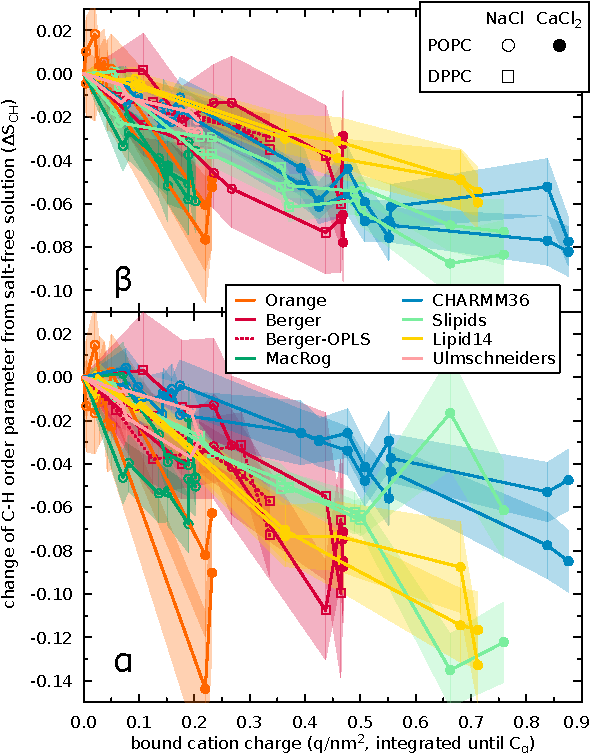
\includegraphics[width=8.6cm]{../Fig/dOP_vs_boundCationCharge_Ca.pdf}
  \caption{\label{electrometer_ca}
    Change of order parameters (from salt-free solution) of the $\beta$ and $\alpha$ segments,
    $\Delta S_{\rm{CH}}^{\beta}$ and $\Delta S_{\rm{CH}}^{\alpha}$,
    shown as a function of bound cation charge.
    The order parameters as well as the bound charge calculated separately for
    each leaflet; {\bf cations residing between the bilayer centre and the density maximum of $\alpha$ carbon
    considered bound}; error bars (shaded) show the standard error of the mean over all lipids.
    }
\end{figure}

Figures~\ref{electrometer_g3},~\ref{electrometer_ca} and~3 in the main text show that in all MD models a clear correlation existed between the bound cation charge and the change of the ($\beta$, $\alpha$) order parameters. Also, this correlation did not seem to depend heavily on ion type, as Na$^+$ and Ca$^{2+}$ fell effectively on the same line in each force field.
In other words, the plots demonstrate that the molecular electrometer is robust, that is, qualitatively reproduced also in MD simulations, and even with rather inaccurate force fields. (A similar robust effect was found to be the reorientation of the PC headgroup upon dehydration in our previous paper~\cite{botan15}.)

We wish to note that with the mono- and divalent ions the bound charge is localised differently in the membrane.
Interestingly, however, a single linear slope could capture responses to both (Figs.~\ref{electrometer_g3},~\ref{electrometer_ca} and 3 in the main text).
This is somewhat surprising, as one might expect correlation effects between the bound ions;
these might become evident only at higher concentrations.

%We also note that the differences between force fields for order parameter changes as a function of bound charge do not seem to exactly match the differences between force fields for order parameter changes as a function of ion concentration (Fig.~\ref{ordPions}): The order parameter change as a function of bound charge is similar e.g. for Lipid14 and Berger even though significant difference is observed as a function of ion concentration, and Orange has the smallest dependence on ion concentration but strongest dependence on bound cation charge. Conclusion seems to be that in most cases the order parameter changes as a function of ion concentration arise from differences in ion binding affinity, not from different headgroup responses to ion binding. HOWEVER. The slopes are affected by the choice of the integration limit (see Figs.~\ref{electrometer_g3},~\ref{electrometer}, and \ref{electrometer_ca}), so one should be very careful with conclusions.
%The exception may be the alpha carbon for CHARMM. It has the weakest dependence on bound charge and it is the only segment which agrees with experiments as a function of Calcium concentration. It may be that CHARMM is more realisitic in this aspect --- or this might coincidental.




\section{Headgroup response to charged amphiphiles}

As discussed in the previous section, the definition of bound ions is somewhat arbitrary in simulations. Therefore, for systems with ions
the order parameter changes as a function of the bound charge cannot be straightforwardly
compared between simulations and experiments.
In systems with charged
amphiphiles the situation is more straightforward, because all the charges can be assumed 
to be located in the bilayer in both simulations and experiments.

Figure~\ref{DMPC_DMTAP} shows the order parameter changes versus
the number of charged amphiphiles per PC lipid, calculated from previously published simulation 
data~\cite{miettinen09,DMPC_DMTAP0mol,DMPC_DMTAP6mol,DMPC_DMTAP50mol} and
experiments~\cite{scherer89,franzin98}.
\begin{figure}[t]
  \centering
  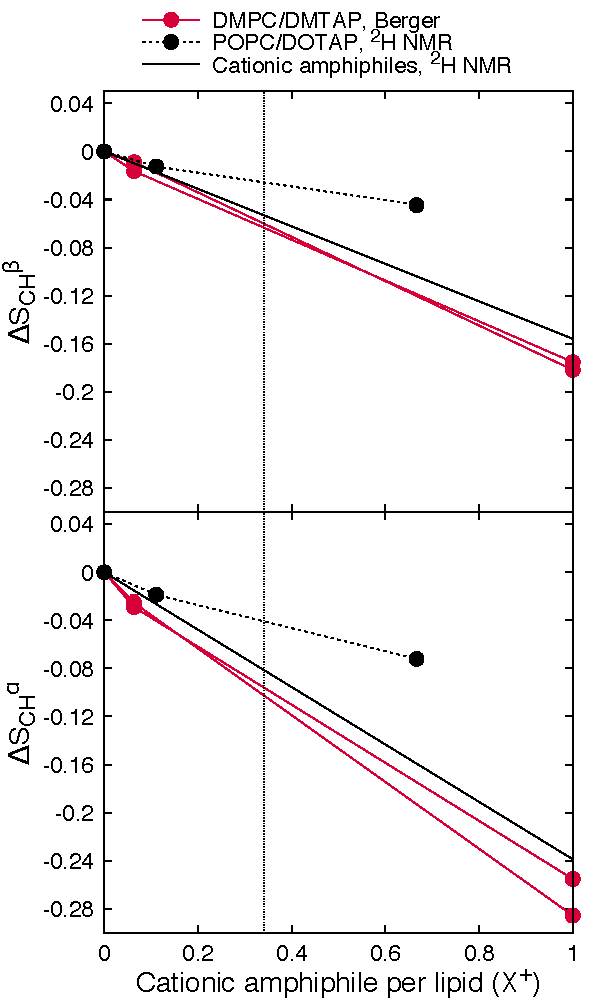
\includegraphics[width=8cm]{../Fig/OrderParameterDMPC_DMTAP.pdf} 
  \caption{\label{DMPC_DMTAP}
    Order parameter changes as a function of number of cationic amphiphiles per PC lipid from simulations~\cite{miettinen09,DMPC_DMTAP0mol,DMPC_DMTAP6mol,DMPC_DMTAP50mol} 
    and experiments~\cite{scherer89,franzin98}. Experimental points for binary mixtures of POPC and DOTAP (1,2-dioleoyloxy-3-(trimethylammonio)propane)
    are from Ref.~\citenum{franzin98}. The solid experimental lines are $\Delta S_{\rm{CH}}^{i}=\frac{4}{3}\chi^{-1}m_i X^\pm$, where $m_i$ are the averages
    over the different amphiphiles measured in Ref.~\citenum{scherer89}.
}
\end{figure}
The experimental data from various amphiphiles with saturated acyl chains~\cite{scherer89} had a
steeper slope than the experimental data from POPC/DOTAP (1,2-dioleoyloxy-3-(trimethylammonio)propane) mixtures~\cite{franzin98}.
The origin of the difference is unknown, but may arise, e.g., from the differences in acyl chain saturation levels, or from differences in the charged amphiphile headgroups.

In the simulations, a Berger-based model was used for binary mixtures of zwitterionic (neutral) dimyristoylphosphatidylcholine (DMPC)
and cationic dimyristoyltrimethylammoniumpropane (DMTAP), with Cl$^-$ counter ions~\cite{miettinen09,DMPC_DMTAP0mol,DMPC_DMTAP6mol,DMPC_DMTAP50mol}. 
The amphiphile acyl chains were fully saturated as in the experimental data for various 
amphiphiles from Ref.~\citenum{scherer89}, whereas the amphiphile headgroup was the same as in the experimental data 
from Ref.~\citenum{franzin98}. The order parameter changes in simulations exceeded the changes measured in Ref.~\citenum{franzin98}
(especially with larger amphiphile concentrations), but were in good agreement with Ref.~\citenum{scherer89}. That said, the simulated
system was not exactly the same as in the experiments, and also the potential effect of Cl$^-$ binding affinity could not be excluded.
Thus, with the available data we could not accurately determine how realistic the headgroup response to bound charge was in these simulations. 

To estimate the maximum error, we took the maximum amount of bound cation charge from Fig.~\ref{electrometer_ca} ($\approx0.5\frac{\rm e}{\rm nm^2}$;
note that the amount would be the same from Fig.~3 in the main text, because practically the whole bound cation peak was inluded already there, see
the Berger panels of Figs.~4 and~6 in the main text),
and assumed an area per lipid of 0.68~nm$^2$. This gave for the maximum amount of bound 
charge per lipid $X^+_{\rm max}=0.5\frac{\rm e}{\rm nm^2}\cdot 0.68\frac{\rm nm^2}{\rm lipid}=0.34\frac{\rm e}{\rm lipid}$,
which is shown as a dashed vertical line in Fig.~\ref{DMPC_DMTAP}. The difference between the simulated and
the farther experimental curve at this point provided estimates for the maximum
overestimation of order parameter decrease: $\approx0.04$ for the $\beta$ and $\approx0.06$ for the $\alpha$ order parameter.
(Note that smaller amounts of bound cations result in smaller numbers.)
These values could, in principle, explain the observed overestimated order parameter changes in the Berger model due to CaCl$_2$, but not the ones due to
NaCl (see Fig.~2 in the main text).

In conclusion, with the current data we cannot fully exclude the possibility that the overestimated order parameter response to
CaCl$_2$ in the Berger model arose from an oversensitive headgroup response to bound cations. However, in the presence of NaCl
the differences between responses in simulations and experiments in Fig.~2 in the main text were larger than the maximum estimated 
influence from a possible oversensitivity of the headgroup. 

\section{Density distributions with different CaCl$_2$ concentrations}

The density distributions with all simulated CaCl$_2$ concentrations are shown in Fig.~\ref{CAdensities}.
\begin{figure}[t]
  \centering
  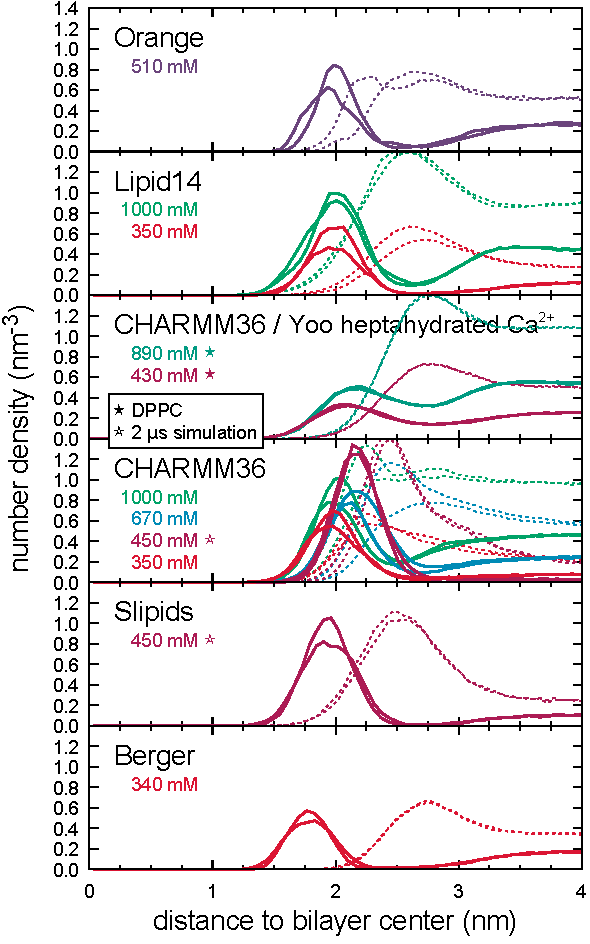
\includegraphics[width=8.6cm]{../Fig/CaDensities_allForSI.pdf}
  \caption{\label{CAdensities}
    Number density profiles of Ca$^{2+}$ (solid lines) and Cl$^-$ (dashed) ions in simulations with different force fields 
    and CaCl$_2$ concentrations. 
%    Figure discussed in https://github.com/NMRLipids/lipid\_ionINTERACTION/issues/4.
  }
\end{figure}

\section{Effect of ion model and polarization}

\begin{figure*}[t]
  \centering
  \includegraphics[width=16cm]{../Fig/OrderParameterIONSchangesSCALED.eps} 
  \caption{\label{OPchangesSCALED}
    The effect of charge scaling~\cite{leontyev11,kohagen14} and NBFIX~\cite{venable13} on order parameter changes in simulations. 
    }
\end{figure*}

It has been suggested that the missing electronic polarizability 
can be compensated by scaling the ion charge in simulations~\cite{leontyev11}. 
To test if this would improve the Na$^+$ ion binding behaviour, we ran simulations with Berger-DPPC-97, BergerOPLS-DPPC-06
and Slipids with scaled Na$^+$ and Cl$^-$ ions. For Berger-DPPC-97 and BergerOPLS-DPPC-06 models 
the ion charge in systems listed in Table~1 in the main text was simply scaled with 0.7 and
the related files are available 
at ~\cite{DPPCBergerNaCl150mMscaled,DPPCBergerNaCl1000mMscaled,DPPCBergerOPLS06NaCl150mMscaled,DPPCBergerOPLS06NaCl1000mMscaled}). 
For simulations with Slipids the electronic continuum correction (ECC) ion model by Kohagen et al. was used~\cite{kohagen16} and the related files are 
available at~\cite{slipidsFILESpopcSCALED}. The simulation parameters were identical to those employed in the simulation of POPC with 130~mM NaCl (see Methods).
The order parameter changes (Fig.~\ref{OPchangesSCALED}) and Na$^+$-binding affinity (Fig.~\ref{NAdensitySCALED}) are decreased by the charge scaling but 
yet overestimated with respect to the experiments. Thus the overestimated binding affinity cannot be fixed by only scaling the charges of ions.

\begin{figure}[h]
  \centering
  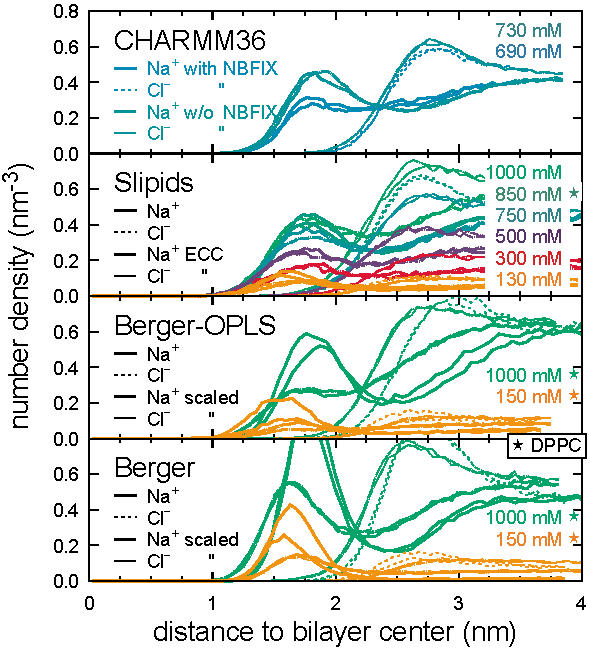
\includegraphics[width=8.6cm]{../Fig/NaDensities_scaledions.pdf} 
  \caption{\label{NAdensitySCALED}
    Number density profiles along membrane normal for Na$^+$ and Cl$^-$ ions. 
    The top panel shows the effect of NBFIX~\cite{venable13} on CHARMM36 simulations;
    other panels show the effect of ion models with scaled charges.
}
\end{figure}

The ion model for CaCl$_2$ with electronic continuum correction (ECC) scaled charges~\cite{kohagen14} was tested with CHARMM36 and Slipids models.
The related files are available at Refs.~\citenum{charmmFILESpopc450mMcaclSCALED} and~\citenum{slipidsFILESpopc450mMcaclSCALED},
respectively, and the results are shown in Figs.~\ref{OPchangesSCALED} and~\ref{CAdensitySCALED}.
The results with scaled charges are slightly improved but yet far from experiments.

\begin{figure}[h]
  \centering
  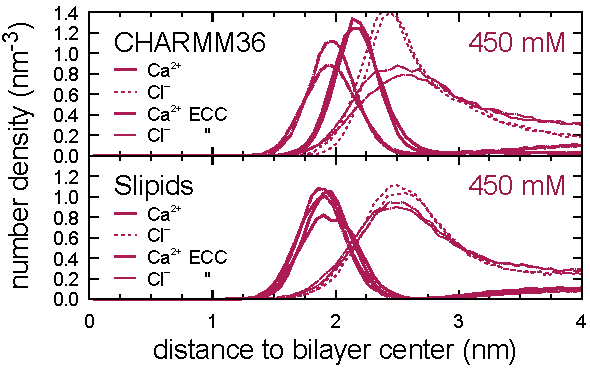
\includegraphics[width=8.6cm]{../Fig/CaDensities_scaledions.pdf} 
  \caption{\label{CAdensitySCALED}
    Number density profiles along membrane normal for Ca$^{2+}$ and Cl$^-$ ions. 
    The effect of ion models with (ECC~\cite{kohagen16}) scaled charges.
}
\end{figure}

Also the effect of NBFIX~\cite{venable13} on Na$^+$ binding in CHARMM36 is quantified.
The simulation data without NBFIX is available at~\cite{charmmPOPC350mMNaClnoNBFIXfiles}.
As expected, Figs.~\ref{OPchangesSCALED} and ~\ref{NAdensitySCALED} show 
more significant order parameter decrease and higher Na$^+$ binding affinity
without NBFIX. Thus, also the CHARMM36 model without NBFIX overestimates the
Na$^+$ binding in PC bilayer.

%I commented this out since the evidence on relation between order parameter change arising from cation binding
%is already quite strong in the manuscript.
%Because the difference promoted by NBFIX~\cite{venable13} is mainly a reduced Na$^+$ density in the headgroup region of the phospholipids,
%this behaviour suggests that it is the direct interaction between the lipids and the Na$^+$ cation 
%(and to no or much lesser extent Cl$^-$ anions) that drives the changes of the order parameters. 


\section{Methods}

\subsection{Simulated systems}
All simulations are ran with a standard setup for planar lipid bilayer in zero tension
with periodic boundary conditions with Gromacs (version numbers 4.5-X-5.0.X)~\cite{pronk13,abraham15} 
or NAMD~\cite{NAMD} software packages.

For the ease of the interested reader in repeating most of the analysis
presented in this Electronic Supplementary Information as well as in the
main text, the centered simulation trajectories, as well as the relevant input
files are provided in a single Zenodo upload at
\url{http://dx.doi.org/10.5281/zenodo.167336}.

\subsection{Analysis}
The order parameters were calculated from simulation trajectories directly applying the equation
$S_{{\rm CH}}=\langle \frac{3}{2}  \cos^2 \theta-\frac{1}{2} \rangle$,
where $\theta$ is the angle between a given C--H bond and the bilayer normal, and the average is taken
over all lipids and time frames. For united atom models, the positions of hydrogen atoms
were calculated for each molecule in each frame \textit{a posteriori} by using the {\it g\_protonate} tool in 
Gromacs 4.0.2 \cite{gromacsMANUAL402}. 
The statistical error in the order parameter was estimated by calculating the average value separately for each lipid molecule,
and then the average and standard error of the mean over the ensemble of lipids (as done also in previous work \cite{botan15}).
All the scripts used for analysis and the resulting data are available in the GitHub repository \cite{githubIONpaper}

\subsection{Simulation details}

\subsubsection{Berger}
{\it POPC:} The simulation without ions is the same as in Ref.~\citenum{ferreira13} and the files are available at Ref.~\citenum{bergerFILESpopc}. 
The starting structures for simulations with ions is made by replacing water molecules with appropriate amount of ions (see Table~1 in the main text).
The Berger force field was used for the POPC~\cite{berger97}, with the dihedral potential next to the double bond 
taken from~\cite{bachar04}. The ion parameters from ffmgx~\cite{straatsma88} were used.
Timestep of 2~fs was used with leap-frog integrator. Covalent bond lengths were constrained with LINCS algorithm~\cite{hess97,hess07}. 
Coordinates were written every 10~ps. PME~\cite{darden93,essman95} with real space cut-off at 1.0~nm was used 
for electrostatics. Plain cut-off was used for the Lennard-Jones interactions with a 1.0~nm cut-off.
The neighbour list was updated every 5th step with cut-off at 1.0~nm. Temperature was coupled separately
for lipids, water and ions to 298~K with the velocity-rescale method~\cite{bussi07} with coupling constant 0.1~ps$^{-1}$.
Pressure was semi-isotropically coupled to the atmospheric pressure with the Parrinello--Rahman barostat~\cite{parrinello81}.

{\it DPPC:} The simulation without ions is the same as in~\cite{botan15} and the files are available at~\cite{bergerDPPCfiles}.
The initial configuration contained 72 DPPC lipids and 2880 SPC water molecules.
The standard Berger DPPC force field was used ~\cite{berger97} (simulations indicated as Berger-DPPC-97 in Table~1 in the main text). 
The electrostatics were handled with PME~\cite{darden93,essman95}, with real-space Coulomb cut-off set at 1.0 nm. Lennard-Jones potentials were cut off at 1.0 nm. The neighbour list for all non-bonded interactions was updated every 10 steps. 
Temperature was set to 323K with the velocity-rescale method~\cite{bussi07} using a coupling constant of 0.1 ps$^{-1}$.  Semi-isotropic pressure coupling at 1 atm was handled with the Parrinello-Rahman barostat~\cite{parrinello81} with 1 ps coupling constant. The time step was 4 fs, and coordinates were written every 10 ps. The total simulation time was 120 ns (without pre-equilibration) and last 60 ns was used in the order parameter analysis. 

For simulations with added salt, the appropriate number of SPC water molecules were randomly replaced with ions. Ions were described by the ffgmx parameters \cite{straatsma88}. In simulations with scaled charges, charge-scaling was applied by scaling the ion charges  by a factor 0.7. Conditions in the ion simulations were as with the pure DPPC described above. The duration of the simulations was 120 ns (without pre-equilibration) and last 60 ns was used in the order parameter analysis.

All the simulation files for pure DPPC simulations can be found at Ref.~\citenum{bergerDPPCfiles} and for the simulations with ions 
at Refs.~\citenum{bergerDPPC150mMfiles, bergerDPPC1000mMfiles} 
and with scaled ions at Refs.~\citenum{DPPCBergerNaCl150mMscaled, DPPCBergerNaCl1000mMscaled}.



\subsubsection{BergerOPLS}
For simulations without ions, the initial configuration contains 72 DPPC lipids and 2880 SPC water molecules. For simulations with added salt, the appropriate amount of SPC water molecules were randomly replaced with ions. The number of ions is reported in Table~1 in the main text.
For the lipids, we used the same version of Berger force field as in previous simulations, described in \cite{berger97}; for the ions, we used the \r{A}qvist parameters \cite{aqvist90} (commonly used within the OPLS-AA force field). Issues related to the compatibility between Berger and OPLS-AA force fields are described in ref.~\cite{tieleman06}. 
A set of simulations was carried out using reduced electrostatic charges on the ions; in this case, a charge of 0.7 e was used on the ions, as described in refs.~\cite{kohagen16, leontyev11}. Except for the ion force field, all simulation parameters (for non-bonded interactions, integration time step, thermostat, etc.) were identical to the parameters used in the Berger DPPC simulations described above.

All simulation files can be found at Ref.~\citenum{bergerOPLSDPPCfiles} for pure DPPC simulations, 
at Refs.~\citenum{bergerOPLSDPPCfiles150mMnacl, bergerOPLSDPPCfiles1000mMnacl} for simulations with ions,
and at Refs.~\citenum{DPPCBergerOPLS06NaCl150mMscaled, DPPCBergerOPLS06NaCl1000mMscaled} for simulations with ions with scaled charges. 



\subsubsection{CHARMM36}
{\it POPC with NaCl:}
The simulation without ions is taken directly from Refs.~\citenum{botan15,charmm36filesSHORT}. 
The starting structures for simulations with NaCl were made by replacing randomly located 
water molecules of the structure of pure POPC simulation with appropriate amount of ions.
The force field for lipid were the same as in Refs.~\citenum{botan15,charmm36filesSHORT}.
The compatible TIP3P parameters for CHARMM36 and ion parameters with NBFIX by Venable et al.~\cite{venable13} were used.
Simulations were ran with Gromacs 4.5.5 software~\cite{pronk13}.
Timestep of 2~fs was used with leap-frog integrator. Covalent bonds with hydrogens were constrained with LINCS algorithm~\cite{hess97,hess07}. 
Coordinates were written every 5~ps. PME with real space cut-off 1.4~nm was used 
for electrostatics. Lennard-Jones interactions were switched to zero between 0.8~nm and 1.2~nm.
The neighbour list was updated every 5th step with cut-off 1.4~nm. Temperature was coupled separately
for lipids and solution to 303~K with the velocity-rescale method~\cite{bussi07} with coupling constant 0.2~ps.
Pressure was semi-isotropically coupled to the atmospheric pressure with the Berendsen method~\cite{berendsen84}.

Simulation without NBFIX~\cite{venable13} was ran with the same settings, except that 
the temperature was kept at 310~K with Nos{\'e}--Hoover~\cite{nose84,hoover85} thermostat 
(simulation files available at Ref.~\citenum{charmmPOPC350mMNaClnoNBFIXfiles}). 

%CaCl_2 simulations by MYKHAILO:
{\it POPC with CaCl$_2$:}
The starting structures with varying amounts of CaCl$_2$ were constructed using the CHARMM-GUI Membrane Builder (http://www.charmm-gui.org/) online tool~\cite{lee15}. 
All runs were performed with Gromacs 5.0.3 software package~\cite{abraham15} and CHARMM36 additive force field parameters for lipids~\cite{klauda10} and ions were obtained from CHARMM-GUI input files. 
Simulation parameters provided by CHARMM-GUI were used.
Particularly, the lengths of the bonds involving hydrogens were constrained with LINCS~\cite{hess97,hess07}. The temperatures of the 
lipids and the solvent were separately coupled to the Nose--Hoover~\cite{nose84,hoover85} thermostat with a target temperature of 303 K and a relaxation time constant of 1.0 ps. Semi-isotropical 
pressure coupling to 1 bar was obtained with the Parrinello-Rahman barostat~\cite{parrinello81} with a time constant of 5 ps. Equations of motion were integrated with the Verlet algorithm~\cite{pall13} 
using a timestep of 2 fs. Long-range electrostatic interactions were calculated using the PME~\cite{darden93,essman95} method with a fourth order smoothing spline. A real space cut-off of 1.2 nm 
was employed with grid spacing of 0.12 nm in the reciprocal space. Lennard-Jones interactions were smoothly switched to zero between 1.0 nm and 1.2 nm. Verlet cutoff-scheme~\cite{pall13}  
was used with the long-range neighbour list updated every 20 steps. Coordinates were written every 10 ps.
After energy minimisation and an equilibration run of 0.5 ns, 200 ns simulations were ran and the last 100 ns of each simulation was employed for the analysis.

 % DPPC + CaCl2 by Sergey Vilov and Claire Loison, 
 % Ca2+ model from  http://dx.doi.org/10.1002/bip.22868 (Jejoong Yoo and Aksimentiev, Oleksii) 
{\it DPPC with CaCl$_2$ (Yoo model):}
The systems contained 128 DPPC lipids and about 7600 TIP3P~\cite{jorgensen83} water molecules,
and an appropriate amount of ions as indicated in  Table~1 in the main text.  
We have used CHARMM36 additive force field parameters for lipids~\cite{klauda10} with compatible TIP3P water model. 
In the calcium model developed recently by Yoo et al.~\cite{yoo16}, 
each cation is decorated by seven hydrating water molecules (with different charges from the usual TIP3P),
which are constrained to remain in its vicinity. The associated parameter files are available
on \url{http://bionano.physics.illinois.edu/CUFIX}. The constraint on the calcium-oxygen distances
was imposed by adding extra bonds through a harmonic potential $V(r) = k(r-r_0)^2$, 
with $r_0=2.25$~\AA~ and $k=10$~kcal$\cdot$mol$^{-1}$$\cdot$\AA$^{-2}$.
 
The starting  configuration of hydrated lipidic bilayers were constructed using {\it packmol} \cite{packmol} 
with a large area per lipid (64~\AA$^{2}$). 
After a first energy minimisation (5000 steps),
varying amounts of Ca$^{2+}$ and Cl$^-$ ions were added  by replacing water molecules,
using the {\it autoionize} plugin of vmd package \cite{hump96},
mentioning explicitly the ion concentration.
Ion placement is random, with the constraint of  minimum 2~\AA~ between ions and lipids,
as well as between any two ions. A second energy minimisation was performed after inserting the ions.
 
All the minimisation and dynamics were conducted using the NAMD package~\cite{NAMD}.
The temperature of the whole system was controlled with Langevin thermostat with a target temperature of 323~K 
and a relaxation time constant of 1~ps.  The modified NAMD version of Nose--Hoover barostat with Langevin dynamics
(piston period of 0.2~ps and piston decay time of 0.05~ps) was used semi-isotropically
for an average target pressure of 1 bar and an average zero surface tension. 
%The ratio of the box length in $x-$ and $y-$ directions was kept fixed to avoid spurious box anisotropy.
%Samuli: This implies from semi-isotropic coupling, right?
The equations of motion were integrated using the multiple time step Verlet r-RESPA algorithm~\cite{pall13}
with a time step of 2~fs, and electrostatic forces calculated only every two time steps. Covalent
bonds between heavy and hydrogen atoms were constrained using SHAKE/RATTLE algorithm.
Long-range electrostatic interactions were calculated using the PME~\cite{darden93,essman95} method 
with a 6-th order smoothing spline and a grid spacing of about 0.1~nm.
A cut-off of 1.2~nm was employed for the Lennard-Jones
interactions, with a force-based switching function for distances beyond 1~nm,
activating the vdwForceSwitching option to ensure NAMD
compatibility with CHARMM force smoothing. Neighbour
lists with a radius of 1.4~nm were updated every 10 timesteps.
Coordinates were written every 20~ps. After energy minimisation, a run of  200~ns simulations was performed,
and the last $\sim$ 170~ns 
of  trajectory was employed for the analysis.
Error bars are defined by $\pm$ the standard error of the mean, 
taking into account the correlation time of the average order parameters 
(200~ps for 430~mM and 400~ps for 890~mM). 


\subsubsection{MacRog}
The simulation parameters are identical to those employed in our earlier study~\cite{botan15} for the full 
hydration and dehydration simulations. The initial structures with varying amounts of NaCl were constructed from an 
extensively hydrated bilayer by replacing water molecules with ions using the Gromacs {\it genion} tool~\cite{gromacsMANUAL}. Even at the highest 
considered salt concentration, the amount of water molecules per lipid after this replacement process was still greater than 50.

\subsubsection{Orange}
The systems contained 72 POPC lipids and 2880 SPC water molecules, and an appropriate amount of ions as indicated in 
Table~1 in the main text.  

For the lipids, we used an unpublished force field coined Orange force field. 
Briefly, this includes most bonded interactions from Berger lipids~\cite{berger97}, 
except for dihedrals which were derived via \textit{ab initio} calculations on small model compounds. 
As in Berger lipids, Lennard-Jones parameters are from OPLS~\cite{jorgensen84,jorgensen86a,jorgensen86b,jorgensen88,briggs91}.
Partial charges were derived on the basis of \textit{ab initio} calculations. 
In simulations with ions, the \r{A}qvist parameters were used~\cite{aqvist90}. 
The electrostatics were handled with PME~\cite{darden93,essman95}, with real-space Coulomb cut-off set at 1.8 nm. 
Lennard-Jones potentials were cut off at 1.8 nm. 
The neighbour lists for the calculation of non-bonded forces were updated every 5 steps.

Temperature was set to 298K with the velocity-rescale thermostat~\cite{bussi07} using a coupling constant of 0.1 ps$^{-1}$, and the pressure was set to 1 
bar using the Berendsen weak coupling algorithm~\cite{berendsen84} (compressibility of 4.5$\cdot$10$^{-5}$ bar$^{-1}$, time constant of 1 ps), coupling separately the x-y dimension and the z dimension to obtain a tensionless system. 
A time step of 2 fs was used for the integration (with the leap-frog algorithm), coordinates were written every 100 ps, 
and the total simulation time was 60 ns. 

Simulation files for pure lipid simulations are found at Ref.~\citenum{orangePOPCfiles} and for the simulations with ions at Refs.~\citenum{orangePOPC140mMNaClfiles,orangePOPC510mMNaClfiles,orangePOPC510mMCaClfiles,orangePOPC1000mMNaClfiles}.


\subsubsection{Slipids}
{\it DPPC:} The simulation without ions from Ref.~\citenum{botan15}, available at Ref.\citenum{slipidsFILES}, was used. 
For the simulation with 150~mM NaCl, the starting DPPC lipid bilayer, which was built with the online CHARMM-GUI~\cite{lee15}
(http://www.charmm-gui.org/), contained 600 lipids hydrated by 30 water molecules per lipid. 

For the simulation with 850~mM NaCl, the configuration from Ref.~\citenum{slipidsFILES} was taken and 
an appropriate amount of water molecules was converted to ions to form a neutral NaCl solution. 
The simulation files are available at Ref.~\citenum{slipidsFILESdppc}. 
%
Ion parameters by Roux~\cite{beglov94,roux96}, TIP3P water model~\cite{jorgensen83} and 
Stockholm lipids (Slipids) parameters~\cite{jambeck12,jambeck12b} for phospholipids were used. 
GROMACS software package version 4.5.5 or 5.0.7~\cite{pronk13} was employed for all simulations. 
After energy 
minimisation and a short equilibration run of 50 ps (time step 1~fs), 100 ns production runs were performed using 
a time step of 2~fs with leap-frog integrator. All covalent bonds were constrained with the LINCS~\cite{hess97,hess07}
algorithm. Coordinates were written every 100 ps. PME~\cite{darden93,essman95} with real space cut-off at 1.0 nm was used for Coulomb 
interactions. Lennard-Jones interactions were switched to zero between 1.0 nm and 1.4 nm. The neighbour 
lists were updated every 10$^\mathrm{th}$ step with a cut-off of 1.6 nm. Temperature was coupled separately for upper and 
bottom leaflets of the lipid bilayer, and for water to 323 K with the Nos\'e-Hoover thermostat~\cite{nose84,hoover85} using 
a time constant of 0.5 ps. Pressure was semi-isotropically coupled to the atmospheric pressure 
with the Parrinello-Rahman~\cite{parrinello81} barostat using a time constant of 10 ps.


{\it POPC:} The simulation without ions from Ref.~\citenum{botan15}, available at Ref.~\citenum{slipidsFILESpopc} was used. \\
{\it POPC with NaCl:}
A POPC bilayer consisting of 200 lipids, hydrated with 45 water molecules per lipid, 
was simulated in the presence of 130 mM NaCl. 
The Slipids model \cite{jambeck12,jambeck12b}
was employed for lipids, the TIP3P model \cite{jorgensen83} for water, and the ion parameters by Smith 
and Dang \cite{smith94} for NaCl. The system was first
equilibrated for 5~ns with a time step of 1~fs after which a 100~ns production run was performed using
a time step of 2~fs. Trajectories were written every 100~ps. The system was kept in a tensionless state at 1~bar 
using a semi-isotropic Parrinello--Rahman barostat \cite{parrinello81} with a time constant of 1~ps. 
The temperature was maintained at 310~K
with the velocity rescaling thermostat \cite{bussi07}. The time constant was set to 0.5~ps for both lipids and 
solvent (water and ions) which were coupled separately. Non-bonded interactions were calculated
within a neighbour list with a radius of 1~nm and an update interval of 10 steps. The Lennard-Jones
interactions were cut-off at 1~nm, whereas PME \cite{darden93,essman95} was employed for long-range electrostatics. 
Dispersion correction was applied to both energy and pressure. All bonds were constrained with the LINCS \cite{hess97,hess07}.
algorithm. \\
{\it POPC with CaCl$_2$:} A POPC bilayer consisting of 200 lipids, hydrated with 45 water molecules per lipid, 
was simulated in the presence of 450 mM CaCl$_2$. The system was ran for 2000~ns and the last 100~ns was used 
for analysis. Other details are as in POPC with NaCl.


\subsubsection{Lipid14}
The starting structures with varying amounts of ions were constructed using the CHARMM-GUI Membrane Builder (http://www.charmm-gui.org/) 
online tool~\cite{lee15}. The GROMACS compatible force field parameters generated in Ref.~\citenum{botan15} and 
available at Ref.~\citenum{lipid14files} were used. 
The TIP3P water model~\cite{jorgensen83} was used to solvate the system and \r{A}qvist \cite{aqvist90} parameters were used for ions.
All runs were performed with Gromacs 5.0.3 software package~\cite{abraham15}
and LIPID14 force field parameters for POPC~\cite{dickson14}. 

H-bond lengths were constrained with LINCS~\cite{hess97,hess07}. The temperatures of the lipids and the solvent were separately coupled to the 
Nose--Hoover~\cite{nose84,hoover85} thermostat with a target temperature of 298.15 K and a relaxation time constant of 0.1 ps. Semi-isotropic pressure 
coupling to 1 bar was obtained with the Parrinello-Rahman barostat~\cite{parrinello81} with a time constant of 2 ps. Equations of motion were integrated 
with the Verlet algorithm~\cite{pall13} using a timestep of 2 fs. Long-range electrostatic interactions were calculated using the PME~\cite{darden93,essman95} method 
with a fourth order smoothing spline. A real space cut-off at 1.0 nm was employed with grid spacing of 0.12 nm in the reciprocal space. 
Lennard-Jones potentials were cut-off at 1 nm, with a dispersion correction applied to both energy and pressure. Verlet cutoff-scheme~\cite{pall13} 
were used with the long-range neighbour list updated every 20 steps. Coordinates were written every 10 ps.

After energy minimisation and an equilibration run of 5 ns, 200 ns production runs were performed and analysed. In case of the CaCl$_2$ systems 
only the last 100 ns of each simulation was employed for the analysis.

\subsubsection{Ulmschneiders}
The starting structures with varying amounts of ions were constructed using the CHARMM-GUI Membrane Builder (\url{http://www.charmm-gui.org}) 
online tool~\cite{lee15}. The force field parameters were obtained from Lipidbook~\cite{domanski10}. The TIP3P water model~\cite{jorgensen83} 
was used to solvate the system.  Additionally, the simulations of ion-free bilayer were repeated with both Verlet and Group cutoff-schemes~\cite{ulmschneiderPOPC0mMNaClfiles}. 
There was no significant difference in headgroup or glycerol backbone order parameters between these cutoff-schemes. All runs were performed with Gromacs 5.0.3 software package~\cite{abraham15}. 
The glycerol backbone order parameters without ions were not the same as reported in the previous study~\cite{botan15}.
The origin of discrepancy was located to the different initial structures which was taken from CHARMM-GUI in this work
and from Lipidbook in the previous work. Since the order parameters with the initial structure from CHARMM-GUI are
closer to the experimental values, the results indicate that the structure available from Lipidbook is stuck to a
state with incorrect glycerol backbone structure, for more discussion see \url{https://github.com/NMRLipids/lipid_ionINTERACTION/issues/8}.

All-bond lengths were constrained with LINCS~\cite{hess97,hess07}. The temperatures of the lipids and the solvent were separately coupled to the Nose--Hoover~\cite{nose84,hoover85} 
thermostat with a target temperature of 298.15 K and a relaxation time constant of 0.1 ps. Semi-isotropic pressure coupling to 1 bar was obtained 
with the Parrinello-Rahman barostat~\cite{parrinello81} with a time constant of 2 ps. Equations of motion were integrated with the Verlet algorithm~\cite{pall13} using a 
timestep of 2 fs. Long-range electrostatic interactions were calculated using the PME~\cite{darden93,essman95} method with a fourth order smoothing spline. 
A real space cut-off at 1.0 nm was employed with grid spacing of 0.12 nm in the reciprocal space. Lennard-Jones potentials were cut-off at 1 nm, 
with a dispersion correction applied to both energy and pressure. Verlet cutoff-scheme~\cite{pall13} were used with the long-range neighbour list updated 
every 20 steps. Coordinates were written every 10 ps. After energy minimisation and an equilibration run of 5 ns, 200 ns simulations were ran and 
the last 100 ns of each simulation was employed for the analysis.


\section{Author Contributions}
\noindent 
{\it Andrea Catte} performed and analysed Slipids DPPC simulation with NaCl. \\
{\it Mykhailo Girych} ran and analysed several simulations (LIPID14, Ulmschneider and CHARMM36+CaCl$_2$). \\
{\it Matti Javanainen} provided data for several lipid and ion models, participated in discussions throughout the project, and supervised the work of JT. \\
{\it Claire Loison} provided results for CHARMM36 DPPC with CaCl$_{2}$ using Yoo's model, and commented on the manuscript. \\
{\it Josef Melcr} performed and analysed Slipids DPPC simulation with NaCl and CHARMM36 POPC simulation without NBFIX, commented on the manuscript, and prepared the Table of Content figure. \\
{\it Markus S. Miettinen} co-designed the project with OHSO.  Provided the Berger DMTAP/DMPC trajectories. Performed the analysis of $\Delta S_\mathrm{CH}$ as a function of bound charge. Prepared Figs.~\,3, 4 and 6. Edited the manuscript. \\
{\it Luca Monticelli} provided parameters for the Orange model and participated in discussions throughout the project. \\
{\it Jukka M{\"a}{\"a}tt{\"a}} ran and analysed several simulations and participated in discussions throughout the project. \\
{\it Vasily S. Oganesyan} performed and analysed Slipids DPPC simulation with NaCl.\\
{\it O. H. Samuli Ollila} co-designed the project with MSM and managed the work. Ran and analysed several simulations. Wrote the manuscript. \\
{\it Joona Tynkkynen } provided results for the MacRog model. \\
{\it Sergey Vilov} provided results for CHARMM36 DPPC+CaCl$_{2}$ with Yoo's model. \\

%\onecolumngrid
%\listoftodos

\bibliography{refs} %You need to replace "rsc" on this line with the name of your .bib file
\bibliographystyle{rsc} %the RSC's .bst file


\end{document}
